\documentclass[10pt,a4paper]{article}
\usepackage[latin1]{inputenc}
\usepackage{amsmath}
\usepackage{amsfonts}
\usepackage{amssymb}
\usepackage{graphicx}
%%% formatting the code
\usepackage{listings}



\usepackage{color}
\lstset{%
	escapeinside={(*}{*)},%
}

\newcommand{\amidstversion}{\input{../../version.txt}}

\lstset{
	frameround=fttt,
%	language=java,
	numbers=left,
	breaklines=true,
	mathescape, 
	columns=fullflexible, 
	basicstyle=\fontfamily{lmvtt}\selectfont,
	keywordstyle=\color{blue}\fontfamily{lmvtt}\selectfont, 
	numberstyle=\color{black}
}
\lstMakeShortInline[columns=fixed]|



\newcommand{\includejavasource}[1]{\lstinputlisting[language=java]{#1}}
\newcommand{\inlinejava}[1]{\lstinline[columns=fixed,language=java]{#1}}

\newcommand{\lang}[1]{}



\usepackage{hyperref}

\begin{document}



\section{Bayesian Networks: Code Examples}\label{sec:bns}

\begin{itemize}
\item \hyperref[sec:bns:datastreams]{Data Streams}
\item \hyperref[sec:bns:randomvars]{Data Streams}
\item \hyperref[sec:bns:models]{Models}
\begin{itemize}
\item \hyperref[sec:bns:models:creating]{Creating BNs}
\item \hyperref[sec:bns:models:creatinglatent]{Creating Bayesian networks with latent variables}
\item \hyperref[sec:bns:models:modif]{Modifiying Bayesian networks}
\end{itemize}

	\item \hyperref[sec:bns:io]{Input/Output}
\begin{itemize}
	\item \hyperref[sec:bns:io:iods]{I/O of data streams}
	\item \hyperref[sec:bns:io:iobn]{I/O of BNs}
\end{itemize}


	\item \hyperref[sec:bns:inference]{Inference}
\begin{itemize}

	\item \hyperref[sec:bns:inference:engine]{The inference engine}
	\item \hyperref[sec:bns:inference:vmp]{Variational Message Passing}
	\item \hyperref[sec:bns:inference:sampling]{Importance Sampling}
\end{itemize}

\item \hyperref[sec:bns:learning]{Learning Algorithms}
\begin{itemize}
	\item \hyperref[sec:bns:learning:batchml]{Maximum Likelihood}
	\item \hyperref[sec:bns:learning:parallelml]{Parallel Maximum Likelihood}
	\item \hyperref[sec:bns:learning:svb]{Streaming Variational Bayes}
	\item \hyperref[sec:bns:learning:parallelsvb]{Parallel Streaming Variational Bayes}
\end{itemize}




\item \hyperref[sec:bns:conceptdrift]{Concept Drift Methods}
\begin{itemize}
	\item \hyperref[sec:bns:conceptdrift:nbayes]{Naive Bayes with Virtual Concept Drift Detection}
\end{itemize}

\item \hyperref[sec:bns:huginlink]{HuginLink}
\begin{itemize}
	\item \hyperref[sec:bns:huginlink:conversion]{Models conversion between AMiDST and Hugin}
	\item \hyperref[sec:bns:huginlink:io]{I/O of Bayesian Networks with Hugin net format}
	\item \hyperref[sec:bns:huginlink:inference]{Invoking Hugin's inference engine}
	\item \hyperref[sec:bns:huginlink:huginTAN]{Invoking Hugin's Parallel TAN}
\end{itemize}



\item \hyperref[sec:bns:moalink]{MoaLink}
\begin{itemize}
	\item \hyperref[sec:bns:moalink:moaclass]{AMIDST Classifiers from MOA}
	\item \hyperref[sec:bns:moalink:moareg]{AMIDST Classifiers from MOA}
\end{itemize}

\end{itemize}


\subsection{Data Streams}\label{sec:bns:datastreams}

In this example we show how to use the main features of a DataStream object. More precisely, we show six different ways of iterating over the data samples of a DataStream object.


\includejavasource{../../../../examples/src/main/java/eu/amidst/core/examples/datastream/DataStreamsExample.java}

\subsection{Data Streams}\label{sec:bns:randomvars}

This example show the basic functionality of the classes Variables and Variable.

\includejavasource{../../../../examples/src/main/java/eu/amidst/core/examples/variables/VariablesExample.java}


\hyperref[sec:bns]{[Back to Top]}\newline 


\subsection{Models}\label{sec:bns:models}

\subsubsection{Creating BNs}\label{sec:bns:models:creating}
In this example, we take a data set, create a BN and we compute the log-likelihood of all the samples of this data set. The numbers defining the probability distributions of the BN are randomly fixed.
\includejavasource{../../../../examples/src/main/java/eu/amidst/core/examples/models/CreatingBayesianNetworks.java}
\hyperref[sec:bns]{[Back to Top]}\newline 

\subsubsection{Creating Bayesian networks with latent variables}\label{sec:bns:models:creatinglatent}
In this example, we simply show how to create a BN model with hidden variables. We simply create a BN for clustering, i.e., a naive-Bayes like structure with a single common hidden variable acting as parant of all the observable variables.
\includejavasource{../../../../examples/src/main/java/eu/amidst/core/examples/models/CreatingBayesianNetworksWithLatentVariables.java}
\hyperref[sec:bns]{[Back to Top]}\newline 

\subsubsection{Modifiying Bayesian networks}\label{sec:bns:models:modif}
In this example we show how to access and modify the conditional probabilities of a Bayesian network model.

\includejavasource{../../../../examples/src/main/java/eu/amidst/core/examples/models/ModifiyingBayesianNetworks.java}
\hyperref[sec:bns]{[Back to Top]}\newline 


\subsection{Input/Output}\label{sec:bns:io}

\subsubsection{I/O of data streams}\label{sec:bns:io:iods}
In this example we show how to load and save data sets from .arff files.

\includejavasource{../../../../examples/src/main/java/eu/amidst/core/examples/io/DataStreamIOExample.java}
\hyperref[sec:bns]{[Back to Top]}\newline 

\subsubsection{I/O of BNs}\label{sec:bns:io:iobn}
In this example we show how to load and save Bayesian networks models for a binary file with ".bn" extension. In this toolbox Bayesian networks models are saved as serialized objects.

\includejavasource{../../../../examples/src/main/java/eu/amidst/core/examples/io/BayesianNetworkIOExample.java}
\hyperref[sec:bns]{[Back to Top]}\newline 


\subsection{Inference}\label{sec:bns:inference}

\subsubsection{The inference engine}\label{sec:bns:inference:engine}
This example show how to perform inference in a Bayesian network model using the InferenceEngine static class. This class aims to be a straigthfoward way to perform queries over a Bayesian network model. By the default the \textit{VMP} inference method is invoked.

\includejavasource{../../../../examples/src/main/java/eu/amidst/core/examples/inference/InferenceEngineExample.java}
\hyperref[sec:bns]{[Back to Top]}\newline 


\subsection{Inference}\label{sec:bns:inference}

\subsubsection{Variational Message Passing}\label{sec:bns:inference:vmp}
This example we show how to perform inference on a general Bayesian network using the Variational Message Passing (VMP) algorithm detailed in

 \begin{quotation}
 	Winn, J. M., Bishop, C. M. (2005). Variational message passing. In Journal of Machine Learning Research (pp. 661-694).
 \end{quotation}

\includejavasource{../../../../examples/src/main/java/eu/amidst/core/examples/inference/VMPExample.java}
\hyperref[sec:bns]{[Back to Top]}\newline 



\subsubsection{Importance Sampling}\label{sec:bns:inference:sampling}
This example we show how to perform inference on a general Bayesian network using an importance sampling algorithm detailed in

\begin{quotation}
Fung, R., Chang, K. C. (2013). Weighing and integrating evidence for stochastic simulation in Bayesian networks. arXiv preprint arXiv:1304.1504.
\end{quotation}

\includejavasource{../../../../examples/src/main/java/eu/amidst/core/examples/inference/ImportanceSamplingExample.java}
\hyperref[sec:bns]{[Back to Top]}\newline 


\subsection{Learning Algorithms}\label{sec:bns:learning}
\subsubsection{Maximum Likelihood}\label{sec:bns:learning:batchml}
This other example shows how to learn incrementally the parameters of a Bayesian network using data batches,

\includejavasource{../../../../examples/src/main/java/eu/amidst/core/examples/learning/MaximimumLikelihoodByBatchExample.java}
\hyperref[sec:bns]{[Back to Top]}\newline 


\subsubsection{Parallel Maximum Likelihood}\label{sec:bns:learning:parallelml}
This example shows how to learn in parallel the parameters of a Bayesian network from a stream of data using maximum likelihood.

\includejavasource{../../../../examples/src/main/java/eu/amidst/core/examples/learning/ParallelMaximumLikelihoodExample.java}
\hyperref[sec:bns]{[Back to Top]}\newline 


\subsubsection{Streaming Variational Bayes}\label{sec:bns:learning:svb}
This example shows how to learn incrementally the parameters of a Bayesian network from a stream of data with a Bayesian approach using the following algorithm,

\begin{quotation}
Broderick, T., Boyd, N., Wibisono, A., Wilson, A. C., and Jordan, M. I. (2013). Streaming variational Bayes. In Advances in Neural Information Processing Systems (pp. 1727-1735).
\end{quotation}

In this second example we show a alternative implementation which explicitly updates the model by batches by using the class SVB.

\includejavasource{../../../../examples/src/main/java/eu/amidst/core/examples/learning/SVBByBatchExample.java}
\hyperref[sec:bns]{[Back to Top]}\newline 




\subsubsection{Parallel Streaming Variational Bayes}\label{sec:bns:learning:parallelsvb}
This example shows how to learn in the parameters of a Bayesian network from a stream of data with a Bayesian approach using the parallel version of the SVB algorithm,


\begin{quotation}
	Broderick, T., Boyd, N., Wibisono, A., Wilson, A. C., and Jordan, M. I. (2013). Streaming variational Bayes. In Advances in Neural Information Processing Systems (pp. 1727-1735).
\end{quotation}


\includejavasource{../../../../examples/src/main/java/eu/amidst/core/examples/learning/ParallelSVBExample.java}
\hyperref[sec:bns]{[Back to Top]}\newline 



\subsection{Concept Drift Methods}\label{sec:bns:conceptdrift}
\subsubsection{Naive Bayes with Virtual Concept Drift Detection}\label{sec:bns:conceptdrift:nbayes}
This example shows how to use the class NaiveBayesVirtualConceptDriftDetector to run the virtual concept drift detector detailed in
\begin{quotation}
Borchani et al. Modeling concept drift: A probabilistic graphical model based approach. IDA 2015.
\end{quotation}

\includejavasource{../../../../examples/src/main/java/eu/amidst/core/examples/conceptdrift/NaiveBayesVirtualConceptDriftDetectorExample.java}
\hyperref[sec:bns]{[Back to Top]}\newline 


\subsection{HuginLink}\label{sec:bns:huginlink}
\subsubsection{Models conversion between AMiDST and Hugin}\label{sec:bns:huginlink:conversion}
This example shows how to use the class BNConverterToAMIDST and BNConverterToHugin to convert a Bayesian network models between Hugin and AMIDST formats

\includejavasource{../../../../examples/src/main/java/eu/amidst/core/examples/huginlink/HuginConversionExample.java}
\hyperref[sec:bns]{[Back to Top]}\newline 



\subsubsection{I/O of Bayesian Networks with Hugin net format}\label{sec:bns:huginlink:io}
This example shows how to use the class BNLoaderFromHugin and BNWriterToHugin classes to load and write Bayesian networks in Hugin format

\includejavasource{../../../../examples/src/main/java/eu/amidst/core/examples/huginlink/HuginIOExample.java}
\hyperref[sec:bns]{[Back to Top]}\newline 


\subsubsection{Invoking Hugin's inference engine}\label{sec:bns:huginlink:inference}
This example we show how to perform inference using \href{http://www.hugin.com}{Hugin} inference engine within the AMiDST toolbox

\includejavasource{../../../../examples/src/main/java/eu/amidst/core/examples/huginlink/HuginInferenceExample.java}
\hyperref[sec:bns]{[Back to Top]}\newline 



\subsubsection{Invoking Hugin's Parallel TAN}\label{sec:bns:huginlink:huginTAN}
This example we show how to perform inference using \href{http://www.hugin.com}{Hugin} inference engine within the AMIDST toolbox.\newline 

This example shows how to use \href{http://www.hugin.com}{Hugin}'s functionality to learn in parallel a TAN model. An important remark is that Hugin only allows to learn the TAN model for a data set completely loaded into RAM memory. The case where our data set does not fit into memory, it solved in AMIDST in the following way. We learn the structure using a smaller data set produced by Reservoir sampling and, then, we use AMIDST's ParallelMaximumLikelihood to learn the parameters of the TAN model over the whole data set.\newline 

For further details about the implementation of the parallel TAN algorithm look at the following paper:
\begin{quotation}
Madsen, A.L. et al. A New Method for Vertical Parallelisation of TAN Learning Based on Balanced Incomplete Block Designs. Probabilistic Graphical Models. Lecture Notes in Computer Science Volume 8754, 2014, pp 302-317.
\end{quotation}


\includejavasource{../../../../examples/src/main/java/eu/amidst/core/examples/huginlink/HuginInferenceExample.java}
\hyperref[sec:bns]{[Back to Top]}\newline 



\subsection{MoaLink}\label{sec:bns:moalink}
\subsubsection{AMIDST Classifiers from MOA}\label{sec:bns:moalink:moaclass}

The following command can be used to learn a Bayesian model with a latent Gaussian variable (HG) and a multinomial with 2 states (HM), as displayed in figure below. The VMP algorithm is used to learn the parameters of these two non-observed variables and make predictions over the class variable.

\begin{figure}[h!]
	\centering
	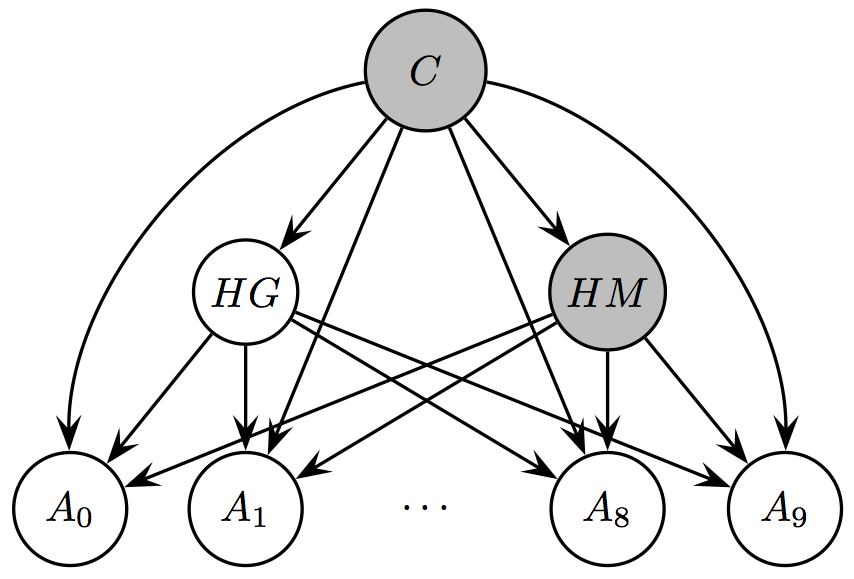
\includegraphics[width=10cm]{img/HODE.jpg}
	\caption{HODE example}
	\label{fig:bns:moalink:HODE}	
\end{figure}

\begin{lstlisting}
java -Xmx512m -cp "../lib/*" -javaagent:../lib/sizeofag-1.0.0.jar 
moa.DoTask EvaluatePrequential -l \(bayes.AmidstClassifier -g 1 
-m 2\) -s generators.RandomRBFGenerator -i 10000 -f 1000 -q 1000
\end{lstlisting}
\hyperref[sec:bns]{[Back to Top]}\newline 




\subsubsection{AMIDST Classifiers from MOA}\label{sec:bns:moalink:moareg}

It is possible to learn an enriched naive Bayes model for regression if the class label is of a continuous nature. The following command uses the model in Figure \ref{fig:bns:moalink:HODEreg} on a toy dataset from WEKA's collection of \href{http://prdownloads.sourceforge.net/weka/datasets-numeric.jar}{regression problems}.

\begin{figure}[h!]
	\centering
	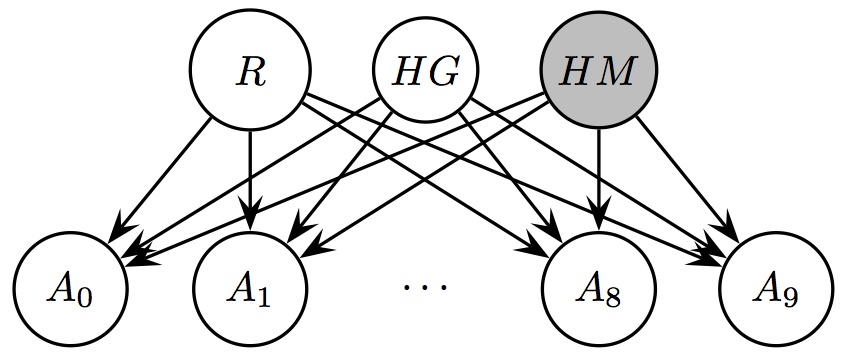
\includegraphics[width=10cm]{img/regressionHODE.jpg}
	\caption{HODE regression example}
	\label{fig:bns:moalink:HODEreg}	
\end{figure}

\begin{lstlisting}
java -Xmx512m -cp "../lib/*" -javaagent:../lib/sizeofag-1.0.0.jar 
moa.DoTask EvaluatePrequentialRegression -l bayes.AmidstRegressor
-s (ArffFileStream -f ./quake.arff)
\end{lstlisting}

Note that the simpler the dataset the less complex the model should be. In this case, \texttt{quake.arff} is a very simple and small dataset that should probably be learn with a more simple classifier, that is, a high-bias-low-variance classifier, in order to avoid overfitting. This aims at providing a simple running example.
\hyperref[sec:bns]{[Back to Top]}\newline 

\end{document}